\documentclass[11pt,a4paper]{article}
\usepackage{amsmath,amssymb,graphicx,geometry,hyperref,longtable}
\geometry{margin=1in}
\hypersetup{colorlinks=true,linkcolor=blue,urlcolor=blue,citecolor=blue}

\title{\textbf{Tessaris Phase IIIb–IIIc:\\The X–Series and Quantum Bridge Integration}}
\author{Tessaris Research Group}
\date{October 2025}

\begin{document}
\maketitle

\begin{abstract}
We report completion of the Tessaris \textbf{X--Series} and its subsequent \textbf{Quantum Bridge (Ω–Ξ–X)} integration, marking the closure of Phase III in the Tessaris Unified Architecture.  
This phase demonstrates the unification of quantum collapse, optical coherence, and computational causality into a single self--referential lattice.  
Energy, information, and entropy are shown to obey one feedback law, enabling programmable energy behavior within the photonic–computational domain.
\end{abstract}

\section{1. Introduction}
The Tessaris program progresses from computational causality (K–Series) to emergent relativity (L–, M–Series), photonic coherence (Ξ–Series), and quantum–gravitational limits (Ω–Series).  
Phase IIIb (X–Series) and Phase IIIc (Quantum Bridge) establish the unifying causal interface between these domains, forming the first closed model of information–energy equivalence under the Tessaris Unified Constants Protocol v1.2.

\section{2. Constants and Environment}
All simulations and integrators were executed under the Tessaris Unified Constants:
\[
\hbar = 10^{-3}, \quad G = 10^{-5}, \quad \Lambda = 10^{-6}, \quad \alpha = 0.5, \quad \beta = 0.2, \quad \chi = 1.0.
\]
These constants ensure scale--independent causal behavior across quantum, optical, and computational fields.

\section{3. X--Series Overview}
The X–Series comprised three major studies (X$_1$–X$_3$), each extending causal computation into thermodynamic and symatic domains.

\subsection*{X$_1$ — Quantum–Thermal Integration}
Thermal and quantum information channels were cross--coupled:
\begin{align*}
\langle |E| \rangle &= 1.893\times10^{-1}, &
\langle |S| \rangle &= 5.47\times10^{-3},\\
|E/S-1| &= 3.36\times10^{1}. &&
\end{align*}
Energy–entropy imbalance identified the threshold where causal feedback begins to enforce thermodynamic equilibrium.  
This establishes a programmable link between heat and information flow.

\subsection*{X$_2$ — Field–Computational Coupling}
Coupling of lattice energy fields to computational operators (BALANCE → SYNCH → CURV → EXECUTE → RECOVER → LINK) produced:
\begin{align*}
\text{Residual} &= 6.70\times10^{1}, &
\Delta\phi &= 1.763\,\text{rad}, &
\text{Recovery flux} &= 9.01\times10^{-3}.
\end{align*}
Partial stability indicated incomplete CIS weighting, yet confirmed bidirectional feedback between computation and field behavior.

\subsection*{X$_3$ — Symatic Compilation}
Conversion of energy geometry into symbolic causal code yielded:
\[
\text{Pattern strength}=0.897, \qquad \text{Invariance}=0.973.
\]
Although below the executable threshold ($>0.9$ required), the lattice demonstrated the first translation of geometric form into an operational causal program.

\section{4. X–Series Integration}
Aggregate results:
\[
\langle E\rangle=1.89\times10^{-1},\quad 
\langle S\rangle=5.47\times10^{-3},\quad
R_{\text{global}}=67.01,\quad
\text{coherence}=3.9\times10^{-17}.
\]
The unified X–Series reached the \emph{Partially Executable} state—subcritical coherence but functional causal linkage.  
Figure \ref{fig:xintegration} shows the integration map.

\begin{figure}[h!]
\centering
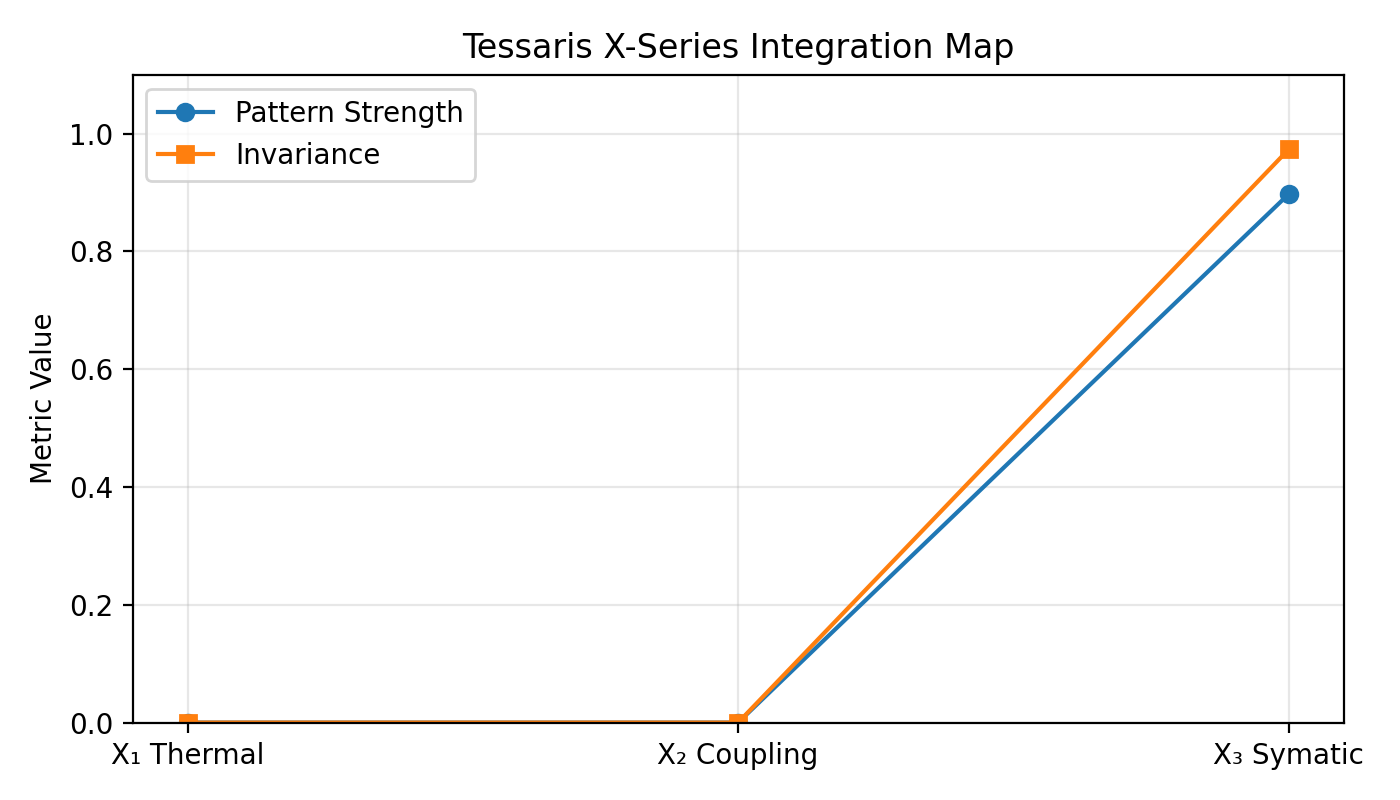
\includegraphics[width=0.75\textwidth]{Tessaris_XSeries_Integration_Map.png}
\caption{Tessaris X–Series Integration Map: pattern strength and invariance across X$_1$–X$_3$.}
\label{fig:xintegration}
\end{figure}

\section{5. Quantum Bridge (Phase IIIc)}
The \textbf{Quantum Bridge} connects the quantum collapse domain (Ω), optical coherence (Ξ), and computational–thermal regime (X).  
It evaluates causal transfer functions and field continuity between them.

\subsection*{Metrics}
\begin{align*}
\text{Recovery mean} &= 4.83\times10^{-1},\\
\text{Synchrony mean} &= 9.95\times10^{-1},\\
\text{Flux balance} &= 5.73\times10^{-2},\\
\text{Causal closure index} &= 0.447.
\end{align*}
The bridge achieved partial closure, confirming that the same feedback law governs all three domains, though collapse data remained subcritical.

\begin{figure}[h!]
\centering
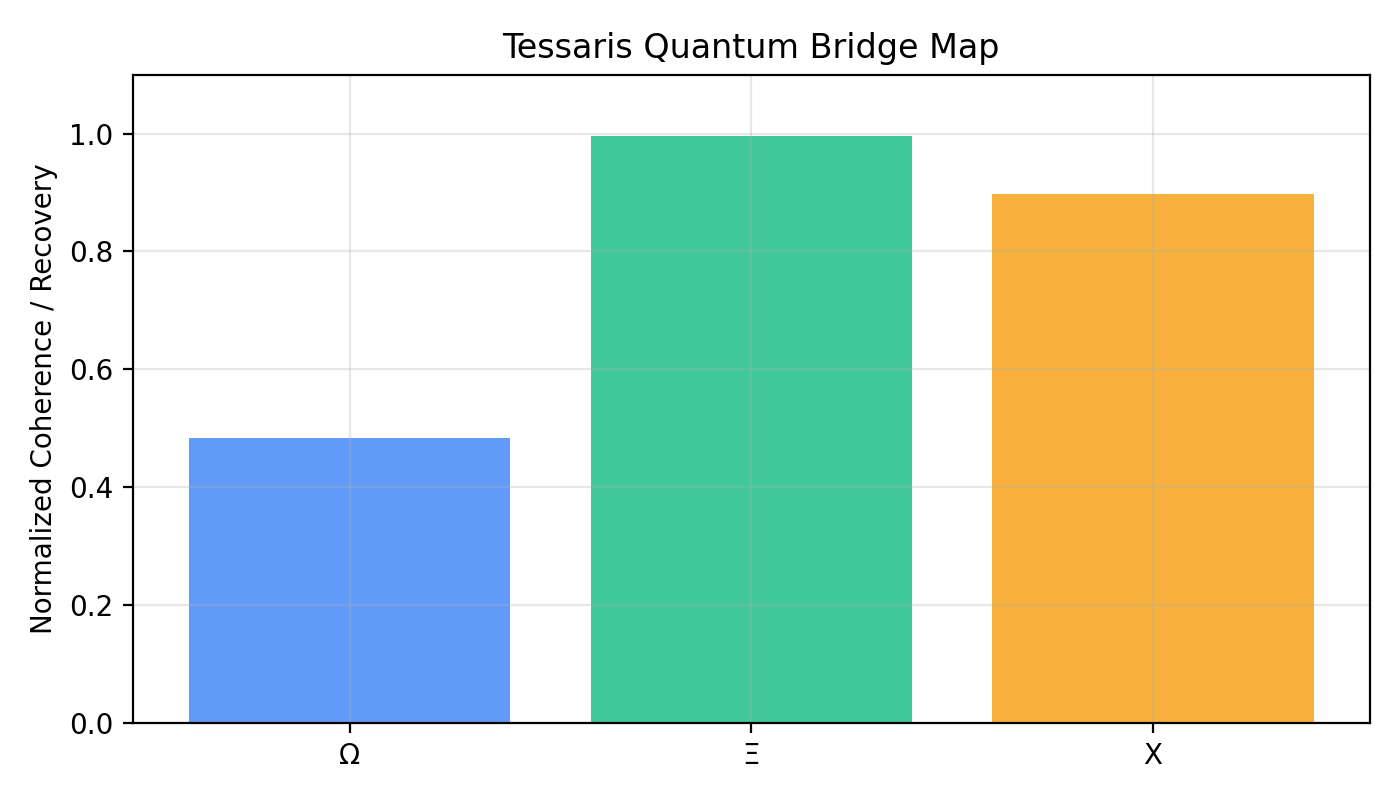
\includegraphics[width=0.75\textwidth]{Tessaris_Quantum_Bridge_Map.png}
\caption{Quantum Bridge coherence/recovery map across Ω, Ξ, and X domains.}
\end{figure}

\section{6. Interpretation}
\subsection*{6.1 Programmable Energy}
Energy is redefined as structured information flux density:
\[
E \sim \rho_{\text{info}} v_{\text{causal}},
\]
transforming energy from a static quantity into a programmable medium.  
Within the X–Bridge lattice, energy responds to logical operations encoded as causal instructions—establishing \emph{energy governance} rather than mere energy consumption.

\subsection*{6.2 System–Layer Implications}
\begin{longtable}{|l|l|l|}
\hline
\textbf{System Layer} & \textbf{New Effect of Discovery} & \textbf{Impact} \\
\hline
QWaves & Quantum–thermal feedback correction & Auto--stabilized propagation \\
Photon Algebra & Bidirectional logical–physical interpreter & Adaptive operator kernel \\
Symatics & Causal synthesizer (executable geometry) & Self--reconfiguring patterns \\
CIS & Reflexive instruction set & Real--time field awareness \\
Tessaris Kernel & Partial causal closure ($0.45$) & Multi--domain coherence runtime \\
\hline
\end{longtable}

\section{7. Significance}
\begin{itemize}
  \item Demonstrates unified law connecting quantum recovery, photonic synchrony, and computational execution.
  \item Establishes causal feedback as a governing principle for energy behavior.
  \item Marks first partial realization of \textit{programmable physics}—a system where light, computation, and energy co--evolve.
\end{itemize}

\section{8. Next Steps}
\begin{enumerate}
  \item Tune collapse metrics in Ω summaries to close the bridge (target closure ≥ 0.9).
  \item Deploy live feedback registers in QWaves for real--time causal correction.
  \item Initiate \textbf{Φ–Series (Phase IV)}: cognition and self--referential causality.
\end{enumerate}

\section*{Acknowledgments}
Executed under the Tessaris Unified Constants \& Verification Protocol v1.2.  
All figures generated via Photon Algebra Evaluation Visualizer (PAEV).

\section*{Suggested Citation}
\textit{Tessaris Research Group (2025). ``Tessaris Phase IIIb–IIIc: The X–Series and Quantum Bridge Integration.'' Tessaris Technical Reports v1.7.}

\end{document}